\section*{États des Processus et Diagramme d'État}

Les processus dans un système d'exploitation passent par plusieurs états fondamentaux, chacun correspondant à une phase différente de leur cycle de vie. Voici les principaux états :

\begin{itemize}
    \item \textbf{EX (Exécution)} : L'état dans lequel le processus est actuellement en cours d'exécution sur le CPU.
    \item \textbf{PR (Prêt)} : L'état dans lequel le processus est prêt à être exécuté, mais attend que le CPU soit libre.
    \item \textbf{BL (Bloqué)} : L'état dans lequel le processus attend la fin d'une opération d'I/O ou un autre événement.
    \item \textbf{EM (En Mémoire)} : L'état dans lequel le processus ou ses parties sont résidents en mémoire principale.
    \item \textbf{HM (Hors Mémoire)} : L'état dans lequel le processus est partiellement ou complètement paginé sur le disque dur.
\end{itemize}

\begin{figure}[h]
    \centering
    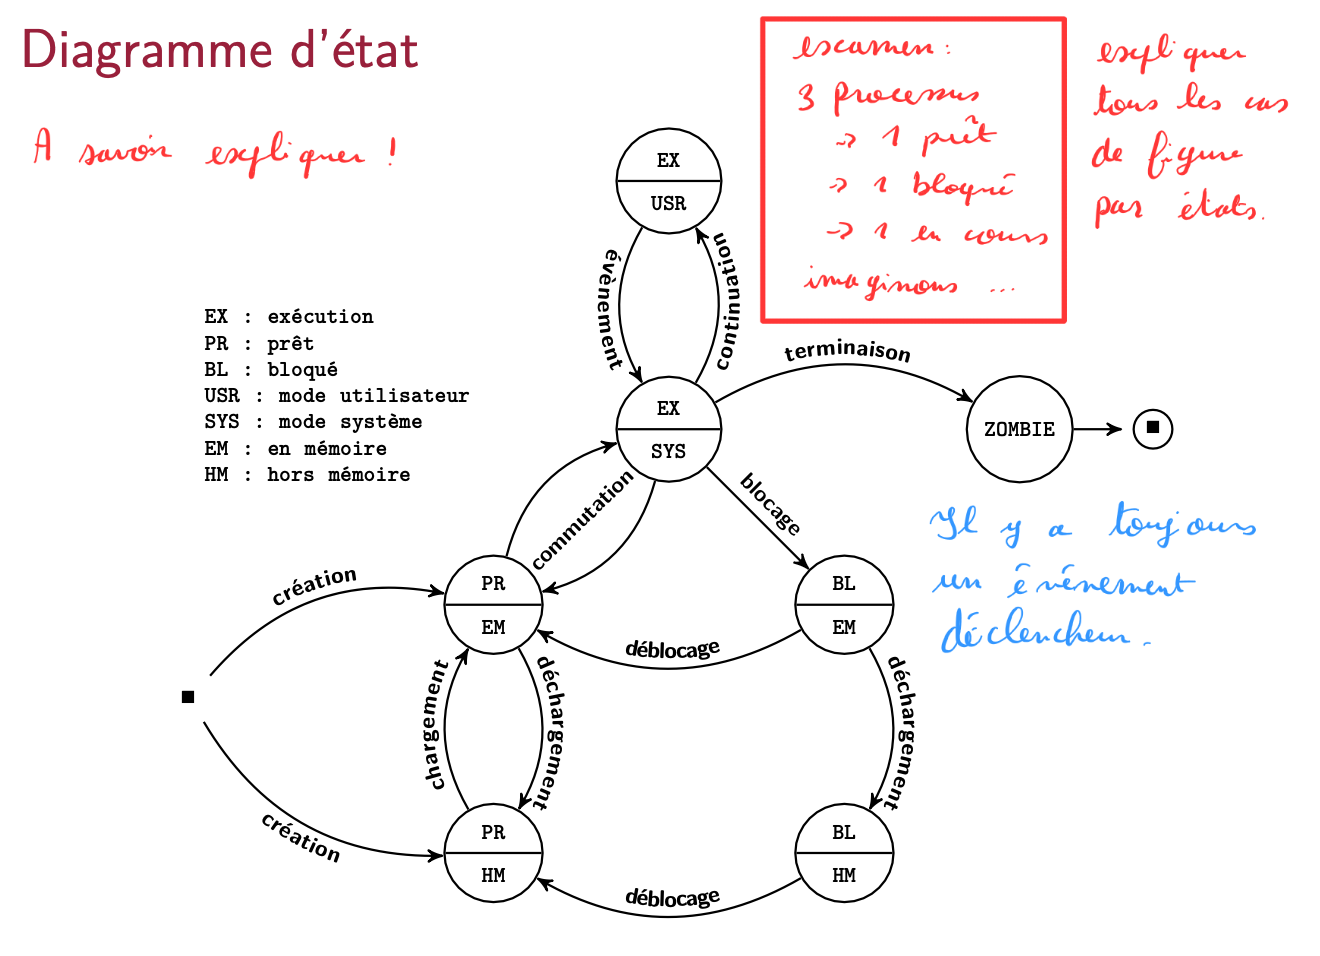
\includegraphics[width=0.8\textwidth]{Images/Diagrams/schema.png}
    \caption{Schéma des états des processus}
\end{figure}

Chaque transition d'un état à un autre peut être déclenchée par divers événements, tels que des interruptions, des appels système, des fautes de pages, etc.

\section*{Cas de Figure avec Trois Processus}

Imaginons trois processus avec les états suivants :

\begin{itemize}
    \item \textbf{P1 (en cours)} : EX (Exécution)
    \item \textbf{P2 (prêt)} : PR (Prêt)
    \item \textbf{P3 (bloqué)} : BL (Bloqué)
\end{itemize}

Nous allons examiner les transitions possibles entre ces états en prenant en compte la protection/projection de la mémoire et la pagination.

\subsection*{1. Transition de P1 (EX) à P2 (PR)}

\textbf{Cause :} Fin du quantum de temps (dans un algorithme de round-robin), ou une interruption I/O.

\subsubsection*{Détails Techniques}

\begin{itemize}
    \item \textbf{Algorithme d'Ordonnancement :} Utilisation de l'algorithme Round-Robin.
    \begin{itemize}
        \item \textbf{Fonctionnement :} L'algorithme Round-Robin assigne un quantum de temps fixe à chaque processus. À la fin de ce quantum, le processus est préempté et le CPU est attribué au processus suivant dans la file d'attente des processus prêts.
        \item \textbf{Exemple :} Si P1 a un quantum de 100 ms, après ces 100 ms, il est préempté et P2 (le prochain dans la file) obtient le CPU.
    \end{itemize}
    \item \textbf{Projection/Protection :} Les tables de pages de P2 sont projetées en mémoire principale (MP) si nécessaire, avec des mécanismes de protection pour assurer que seules les pages de P2 sont accessibles.
    \begin{itemize}
        \item \textbf{Projection :} Projection signifie que les pages virtuelles du processus P2 sont mappées aux cadres de pages physiques en mémoire.
        \item \textbf{Protection :} Les bits de contrôle dans les tables de pages assurent que le processus P2 ne peut accéder qu'à ses propres pages.
    \end{itemize}
    \item \textbf{Pagination :} Si une page nécessaire n'est pas en mémoire, un défaut de page est déclenché, et la page est chargée à partir de la mémoire secondaire.
    \begin{itemize}
        \item \textbf{Défaut de Page :} Se produit lorsque P2 tente d'accéder à une page qui n'est pas actuellement en mémoire principale.
        \item \textbf{Algorithme de Remplacement :} Le système d'exploitation choisit une page à remplacer en utilisant des algorithmes comme LRU (Least Recently Used), FIFO (First In First Out), etc.
    \end{itemize}
\end{itemize}

\textbf{Transition :} P1 passe de EX à PR, P2 de PR à EX.

\textbf{État final :} P1 (PR), P2 (EX), P3 (BL).

\subsection*{2. Transition de P2 (EX) à P3 (BL)}

\textbf{Cause :} P2 demande une opération I/O et doit attendre la fin de cette opération.

\subsubsection*{Détails Techniques}

\begin{itemize}
    \item \textbf{Algorithme d'Ordonnancement :} Le processus suivant prêt à être exécuté est sélectionné (par exemple, P1).
    \begin{itemize}
        \item \textbf{Sélection :} Le système d'exploitation sélectionne P1 (prêt) pour l'exécution, suivant l'algorithme Round-Robin.
    \end{itemize}
    \item \textbf{Projection/Protection :} Les pages de P3 peuvent être projetées en mémoire principale si nécessaires, et les pages de P2 peuvent être déplacées vers le disque.
    \begin{itemize}
        \item \textbf{Projection :} Avant que P3 ne puisse être prêt, ses pages doivent être en mémoire.
        \item \textbf{Protection :} Les tables de pages sont mises à jour pour refléter les nouvelles pages en mémoire.
    \end{itemize}
    \item \textbf{Pagination :} Les pages non utilisées de P2 peuvent être paginées vers le disque.
    \begin{itemize}
        \item \textbf{Déplacement :} Si la mémoire principale est pleine, certaines pages de P2 peuvent être déplacées vers le disque pour faire de la place pour P3.
    \end{itemize}
\end{itemize}

\textbf{Transition :} P2 passe de EX à BL, P1 de PR à EX.

\textbf{État final :} P1 (EX), P2 (BL), P3 (BL).

\subsection*{3. Transition de P3 (BL) à P1 (PR)}

\textbf{Cause :} L'événement attendu par P3 (fin d'une opération I/O) se produit.

\subsubsection*{Détails Techniques}

\begin{itemize}
    \item \textbf{Algorithme d'Ordonnancement :} Le processus suivant prêt à être exécuté est sélectionné.
    \begin{itemize}
        \item \textbf{Sélection :} Une fois l'opération I/O terminée, P3 est déplacé de BL à PR.
    \end{itemize}
    \item \textbf{Projection/Protection :} Les pages de P3 peuvent être projetées en mémoire principale si nécessaires.
    \begin{itemize}
        \item \textbf{Projection :} Les pages nécessaires de P3 sont chargées en mémoire principale si elles ne le sont pas déjà.
    \end{itemize}
    \item \textbf{Pagination :} Si les pages de P3 avaient été paginées, elles sont rechargées en mémoire.
    \begin{itemize}
        \item \textbf{Rechargement :} Les pages qui avaient été déplacées vers le disque pour P3 sont ramenées en mémoire principale.
    \end{itemize}
\end{itemize}

\textbf{Transition :} P3 passe de BL à PR, P1 de EX à PR.

\textbf{État final :} P1 (PR), P2 (BL), P3 (PR).

\section*{Protection/Projection de la Mémoire}

La protection et la projection de la mémoire sont des concepts clés pour garantir que chaque processus accède uniquement à sa propre mémoire. Cela est réalisé grâce aux tables de pages et aux mécanismes de protection matérielle comme les registres de contrôle et les modes de privilège du processeur.

\subsection*{Concepts Clés}

\begin{itemize}
    \item \textbf{Tables de Pages :} Utilisées pour mapper les adresses virtuelles aux adresses physiques.
    \begin{itemize}
        \item \textbf{Fonctionnement :} Chaque entrée de la table de pages contient l'adresse de la page en mémoire principale ou une indication que la page se trouve sur le disque.
    \end{itemize}
    \item \textbf{Mécanismes de Protection :} Utilisation de bits de contrôle pour empêcher les accès non autorisés.
    \begin{itemize}
        \item \textbf{Bits de Contrôle :} Indiquent les permissions de lecture, écriture et exécution pour chaque page.
    \end{itemize}
    \item \textbf{Basculement de Stack :} Lorsqu'une interruption ou un événement se produit, le système peut basculer sur une stack dédiée pour le gestionnaire d'événements.
    \begin{itemize}
        \item \textbf{Fonctionnement :} Le processeur sauvegarde le contexte du processus courant et utilise une stack spéciale pour gérer l'interruption, garantissant que la stack du processus est protégée.
    \end{itemize}
\end{itemize}

\section*{Pagination}

La pagination est utilisée pour gérer la mémoire de manière efficace, en divisant la mémoire en blocs de taille fixe appelés pages. Lorsque la mémoire physique est pleine, certaines pages peuvent être déplacées vers le disque dur (mémoire secondaire).

\subsection*{Concepts Clés}

\begin{itemize}
    \item \textbf{Défaut de Page :} Se produit lorsqu'une page demandée n'est pas en mémoire. Le système doit alors charger cette page à partir du disque, ce qui peut entraîner une transition d'état.
    \begin{itemize}
        \item \textbf{Gestion du Défaut de Page :} Le gestionnaire de mémoire localise la page manquante sur le disque, la charge en mémoire principale, et met à jour les tables de pages.
    \end{itemize}
    \item \textbf{Algorithmes de Remplacement de Pages :} LRU (Least Recently Used), FIFO (First In First Out), NRU (Not Recently Used), et Seconde Chance. Ces algorithmes déterminent quelles pages doivent être remplacées lorsqu'une nouvelle page doit être chargée.
    \begin{itemize}
        \item \textbf{LRU :} Remplace la page qui n'a pas été utilisée depuis le plus longtemps.
        \item \textbf{FIFO :} Remplace la page la plus ancienne.
        \item \textbf{NRU :} Remplace une page qui n'a pas été récemment utilisée.
        \item \textbf{Seconde Chance :} Modifie FIFO en donnant une seconde chance aux pages qui ont été référencées récemment.
    \end{itemize}
\end{itemize}

\section*{Diagramme d'État avec Cas de Figure}

Un diagramme d'état peut être utilisé pour illustrer ces transitions. Chaque état et transition doit être clairement indiqué avec les événements correspondants qui déclenchent les transitions.

\subsection*{Exemple de Transitions}

\begin{itemize}
    \item \textbf{EX à PR :} Fin de quantum, interruption.
    \item \textbf{PR à EX :} Sélection par l'ordonnanceur.
    \item \textbf{EX à BL :} Demande I/O.
    \item \textbf{BL à PR :} Fin d'une opération I/O.
\end{itemize}

\section*{Conclusion}

Cette explication couvre les transitions d'état des processus en tenant compte des algorithmes d'ordonnancement, de la protection/projection de la mémoire, et de la pagination. Chaque transition est déclenchée par des événements spécifiques, et la gestion de la mémoire est cruciale pour assurer une exécution efficace et sécurisée des processus. Les algorithmes de remplacement de pages jouent un rôle clé dans la gestion de la pagination pour optimiser l'utilisation de la mémoire physique disponible.
